\documentclass{article}
\usepackage{xcolor}
\usepackage{fullpage}
\usepackage{graphicx}
\usepackage{epstopdf}
\usepackage{caption}
\usepackage{verbatim}
\usepackage{amssymb}
\usepackage{amsmath,amsthm}
\usepackage{amsfonts}
\usepackage{enumerate}
\usepackage{enumitem}
\usepackage{booktabs}
\usepackage{listings}
\usepackage{qtree}
\usepackage{tikz}
\usepackage{bm}
\usepackage{frame,color}
\usepackage{datetime}
\usepackage{etoolbox}
\usepackage{emerald}
\usepackage[T1]{fontenc}
\usepackage{fancyhdr}
\usepackage[hmarginratio=1:1,top=32mm,columnsep=20pt,left=11mm]{geometry} % Document margins
\usepackage{booktabs} % Horizontal rules in tables
\usepackage{hyperref} % For hyperlinks in the PDF
%\usepackage{paralist} % Used for the compactitem environment which makes bullet points with less space 
\usepackage{abstract} % Allows abstract customizationbetween them
\makeatletter
\patchcmd{\chapter}{\if@openright\cleardoublepage\else\clearpage\fi}{}{}{}
\makeatother
\definecolor{shadecolor}{rgb}{184,184,184}
\lstset{language=Matlab,
        frame = single,
        breaklines=true
}
\usetikzlibrary{calc,positioning}
\usetikzlibrary{arrows,automata}
\renewcommand{\familydefault}{\sfdefault}
\fancyhead{} % Blank out the default header
\fancyhead[C]{Project assistU $\bullet$ TI3800 $\bullet$ TU Delft Library} % Custom header text
\begin{document}
\thispagestyle{fancy}
%%%%%%%%%%%%%%%%%%%%%%%%%%%%%%%%TITLE PAGE%%%%%%%%%%%%%%%%%%%%%%%%%%%%%%%%%%%%%%%%%%%%%%%%
\begin{figure}
    \begin{minipage}[H]{0.33\textwidth}
		\vspace{0.3cm}
		
\includegraphics[scale=0.8]{img/TUDelftLogo.eps}
	\end{minipage}
	\begin{minipage}[H]{0.34\textwidth}
		\begin{center}
			\fontfamily{lmdh}\selectfont \textcolor{blue}{}
		\end{center}
		
	
	\end{minipage}
	\begin{minipage}[H]{0.33\textwidth}
			\begin{flushright}

				\small{Arnaud Hambenne \qquad 4047575}\\
				\small{Soheil Jahanshahi \qquad 4127617}\\
				

			\end{flushright}
			
	\end{minipage}
\end{figure}


\begin{minipage}[H]{\textwidth}
\vspace{0.3cm}
		\begin{center}
		
		\vspace{0.3cm}
			\large{\fontfamily{lmr}\selectfont Title fo Document}\\
		\vspace{0.3cm}	
		
		\vspace{0.7cm}	
		\end{center}
	\end{minipage}
%%%%%%%%%%%%%%%%%%%%%%%%%%%%%%%%%%TITLE ENDS HERE%%%%%%%%%%%%%%%%%%%%%%%%%%%%%%%%%%%%%%%%%%	
%%%%%%%%%%%%%%%%%ALL Sections
\section{Introduction}
  The TU Delft Library is an innovative library that is always looking for a creative solution for the future. They proposed us with a project that is intended to help students and researchers to write a scientific publication. The project entails a software environment in which they are able to plan their process of writing in a calendar, to get suggestions about how to correctly write a scientific publication, and where they can get and give feedback on (un)finished work.
The outline of this research report is as follows: First we explain the problem domain, and provide an analysis. Secondly we state our project's requirements. Based on these requirements we propose a research question that embodies our main objectives, followed by a technical analysis. The final part of this research report provides us with the optimal solution for our problem.
  \section{Problem Domain}
  Within the following section we will describe and analyse what our problem domain is, identify the stakeholders, construct the scope and objectives, and summerize our interview we conducted from the Library's Head of Education Support.

\subsection{Domain Description} % (fold)
\label{sub:problem_description}

The goal of this project is the creation and implementation of a prototype for a `Virtual Assistant', which helps students and researchers to write a report, thesis or dissertation. This Virtual Assistant should provide its users with the ability to choose a layout template, allow for scheduling and feedback, and give suggestions or tips to users about how to write a report, thesis or dissertation.
This project should entail either native desktop software, a web application, or a mobile application. The final product should be released as open source software.

\subsection{Domain analysis} % (fold)

One of the key aspects that need to be well-researched for our project is our domain analysis. The domain analysis basically illustrates all the different types of roles involved with the problem domain (i.e. the stakeholders), and what their interests are. First we list all the stakeholders involved with our domain, secondly we define our scope, and finally we summarize a set of interviews we have conducted with people that embody relevant roles.

\subsubsection{Stakeholders} % (fold)

Below we identify the different stakeholders, which roles they can take, and what their main interests are within our problem domain.

\paragraph{Client: TU Delft Library} The TU Delft Library is the entity that requested this project, and is therefor our client. They expect a prototype of a product that meets their requirements.

\paragraph{Users: Students and Researchers} The use of this product is aimed at students, and researchers, which makes them a subset of our users. They want a product that is easy to use and helps them with writing a report/thesis/dissertation.

\paragraph{Users: Reviewers} The use of this product is also aimed at reviewers, which makes the complementary subset of our users. They also want a product that is easy to use and facilitates them in reviewing a report/thesis/dissertation.

\paragraph{Contributors: Open Source Developers} Our client requested that our final version be released as an open source project. This means that at some point in the future other developers are going to improve upon our product. With this in mind, we have to introduce some design ideals and constraints that will make it easier for them to add code in the future.

\subsubsection{Scope \& Objectives}

The scope of our domain is set for the use-case of students who are writing a Bachelor project final report. One obvious reason for this scope is that this project is also a Bachelor final project, which will also include the process of writing a final report. This means that we will have affinity with the scope, which should imply an advantage within our design. Another reason is that there are plainly too many different cases and subjects within our problem domain to serve all of them accordingly within our deadline.
Our main objective is the creation of an online environment that acts as a support for students who are writing a report/thesis/dissertation. It should provide the students with suggestions, tips, sources and other relevant information. It should provide a platform where there is an interaction between students and their peers or superiors (in this case a teacher, coach or supervisor), and where they can exchange feedback towards each other.

\subsubsection{Interview result analysis} % (fold)

The most challenging part in this project is understanding how we can provide suggestions, tips, sources and other relevant information to students. In order to get a more detailed comprehension of this part within our problem domain, we conducted an interview with Nicole Will. Nicole works for the TU Delft Library as the Head of Education Support, and is also involved with the TULib website, which is an informative website about finding and using scientific information.
We wanted to know what the most valuable pieces of information were that we could provide students with when they write a report. She claimed there were three important parts that we should include, being the module on how to cite\cite{tulib:howtocite}, how to make a reference list, and how to use the APA\cite{tulib:apa} style for your references.
Other than these she also found it useful to provide the students with information on how to find information and articles, how to check for relevance and reliability of sources and what plagiarism is and how to avoid it.



  \section{Research Question}
  The context of this project is to build an application that acts as an virtual assistant to help bachelor students to write their article/report in the correct manner. In order to design a robust and reliable software we need to formulate a research question to do the technical research and to come up with feasible and optimal solution for developing an application prototype.\\

Our coach has advised us to develop a web application, We will assume that this is a good choice of platform, however we will conduct research to find out why is this an ideal choice. \\

Our main question is `How to build a reliable \& robust web application prototype to assist students in order to deliver services to them such that they are able to write an article/report in a correct and efficient manner within the time constraint that is given to them? '


  \section{Project Requirements}
   \subsection{Functional Requirements} % (fold)
\label{sub:functional_requirement}
\begin{enumerate}
	\item Many Users: for each project, multiple participants can join the project, owner/owners of the project will be the administrator of his project. the advisor(e.g teacher) will get special attention from student(administrator) comparing to the other members;
	\item Template: User must chose a template from list or upload its own template
	\item Schedule: Schedule for writing report according to type of the template  (Sub schedule each section e.g introduction , etc).
	\item Propose Suggestions/Tips: The system should be able to suggest tips and information to the user on how to write sections.
	\item Send/Receive Feedback: Feedback on report which will be send by reviewer(or other users) and which will be received by student.
	\item Done/Discard: When a user is done/discarding the suggestion/feedback, he should be able to notify that to the system and all other users. 
	\item Upload Document: Ability to upload the document.
	\item In built Chat mechanism: To track the feedback of advisor and follow up the result of conversations. 
	\item Versioning : keeping track of versions of publications of user.
	\item Logging : save user records in a separate log file for usage analytics.
\end{enumerate}

% subsection functional_requirement (end)
\subsection{Technical Requirements} % (fold)
\label{sub:technical_requirements}
\begin{enumerate}
	\item Mobile Support for Android/IOS
	\item Campus ID authentication: login with TUDelft netid
	\item Open source
 	\item Fully Tested System 
	 
\end{enumerate}


% subsection technical_requirements (end)
\subsection{Usability Requirements} % (fold)
\label{sub:usability_requirements}
\begin{enumerate}
	\item System must be fully functional on modern web browsers
	\item Efficiency of use: System must facilitate efficiency of use for the user by providing information on the fly for the context
	\item Intuitiveness: User Interface must be intuitive and easy to use
\end{enumerate}
% subsection usability_requirements (end)
  \section{Technical Analysis}
  When conducting the research for the problem domain, We have extracted information regarding stakeholders and scope of the project. In this section we will justify our findings on technical choices regarding the deployment of the tools, design and system components. These choices are based on the requirement that is given by the product owner and the extra requirement that we think is necessary for developing a robust software.   

\subsection{Why a web application?}
Nowadays people rely heavily on using the web application. Google maps are good example of such an application, It is a very powerful software that provides to the user so many map features within a web browser, users can travel virtually within a map and can zoom for particular locations. Every time a user asks for specific information, that information is pulled dynamically into the web app.\\
 For our purpose web application is the best choice because users can access their data from various locations on any device because all data is stored online and it works on every device with a web browser. It is also safer to run an application on a web browser because It cannot interfere with programs running on the user's computer and this will lead to better performance of the machine.

\subsection{Objective}
There are various models readily available for the implementation of a web application. The choice of a specific model usually depends on the context and objectives of the project itself. Our current project entails the development of a prototype within a time constraint of 11 to 12 weeks, which persuaded us to use a full stack framework. When we would use a full stack frameword, we should be able to focus solely on techniques that allow us to perform rapid prototyping, generate quality code and provide good documentation all of which meet the clients requirements. The following features should facilitate reaching our objectives during the development phase.

\begin{enumerate}
	\item \textbf{Full stack framework}: a framework that gathers all the libraries and help us with the full development stack.
	\item \textbf{Rapid Prototyping}: enable us to convert client requirement into a rapid prototype so it can be reviewed by client and refined in the next prototype.
	\item \textbf{Scalability}: ability of a system, network, or process to handle a growing amount of work in a capable manner or its ability to be enlarged to accommodate that growth.\cite{wiki:scalability}
	\item \textbf{Reliablity}: ability of a system to function under stated conditions.
\end{enumerate}
\subsection{Project Development Methodology} % (fold)
Among several ways to develop the software Agile stands on top in practice comparing to the others (for example waterfall methodology). Scrum Agile is one of the many in agile processes, Agility (iteration) can solve the disadvantages of other development methodologies like waterfall method. In the waterfall method Development process is sequential where the whole product is tested and presented to the client only at the end; Like this if there is a mistake in the requirements, then the project has to start from scratch again correcting those requirements. Agile methodology allows for changes to be made after the initial planning and hence it is easier to add/remove features. Since Agile is based on Sprint(iteration within fixed time), at the end of each sprint, the project priorities can be evaluated by developer together with the client, This makes it possible to give his/her feedback about the product at the earlier stages.\\
Because of the aforementioned advantages of the scrum, we decided to practice scrum agile methodology for this project. The attributes and roles for people involving in the project are as follows:

\begin{enumerate}
	\item \textbf{Roles}
		\begin{itemize}
			
			\item Product Owner/Dev Team: Arnaud Hambenne
			\item Scrum master/Dev Team: Soheil Jahanshahi
			\item Client: TU Delft Library(Babak Dehghanpour , Nicoleta Nastase )
			\item Coach: Alberto Bacchelli
		\end{itemize}
	\item \textbf{\color{red}{TODO}}	
\begin{itemize}
		\item Sprint : one week iteration
		\item Sprint planning meeting: to set highest priority features for each sprint 
		\item Sprint reflections report: to evaluate the estimated effort with actual effort and to discuss the hurdles by the end of each sprint.
		\item Daily Scrum meeting: time-boxed 15 minutes
		\item Sprint Review Meeting: 15 to 20 minutes, meeting with clients to receive their feedback on the product.
		
\end{itemize} 
\end{enumerate}
\subsection{Architectural Model : MVC}
A design pattern is important to write re-usable and maintainable code. For the Virtual assistant application is best to divide the application into three interconnected parts to separate internal representation of information from information that is presented to users or accepted by them\cite{wiki:mvc}. Such a Design is called MVC pattern which consist of three separate parts namely Model, View and Controller.
\begin{figure}[h]
\centering
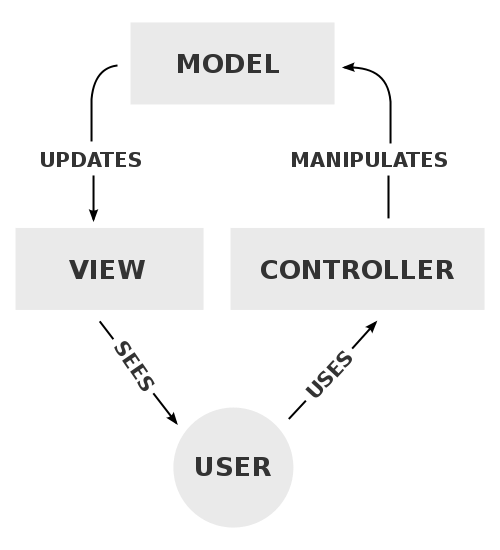
\includegraphics[scale=0.3]{./img/MVC.PNG}
\caption{\small{model,view and controller that are interconnected by directed edges}}
\label{mvc}
	
\end{figure}

As shown in fig \ref{mvc} , MVC will give the application power to separate the classes which are used typically in a database from the user interface; that is necessary to render the model to the user. also controller will act as a brain of the application. controller decides what the user input was and how the model needs to change as a result of that input\cite{codinghorror},controller then respond back to the user by calling resulting view.

\subsection{Choice of framework}
For choosing suitable web application framework we have conducted some  constraint for ourselves to benchmark various popular existing frameworks which is proven in production. Our first criteria was choosing a framework which is based on either Java, Scala, Javascript. With this we have narrowed down our choices to search for the suitable framework. After Analyzing popular frameworks such as \href{https://grails.org/}{Grails}, \href{https://vaadin.com/home}{Vaadin}, \href{https://www.playframework.com/}{Play!} and \href{http://projects.spring.io/spring-framework/}{Spring}. We finally selected two candidates to benchmark them. We boiled down our choices between Spring framework and Play! framework.\\
\subsubsection{Benchmarking}
 below table shows comparison of these two frameworks with constraint that we have settled:\\\\

\begin{center}
	

\begin{tabular}{ |l||l|p{7cm}|p{6cm}|  }
 \hline
 \multicolumn{4}{|c|}{\textbf{Benchmark Table}} \\
 \hline
 ~ & \textbf{Constraint} & \textbf{Play! Framework} & \textbf{Spring Framework}\\
 \hline
 1   & Development Principles & Convention over configuration,Don't repeat yourself,Test-driven development & Convention over configuration,Don't repeat yourself,Test-driven development ,Domain Driven Design   \\
 \hline
 2 & Design pattern & Model-View-Controller,Dependency-injection,Active-Record,DAO,Actors & Model-View-Controller,Dependency-injection,Domain-Driven-Design \\
 \hline
 3 &Operating System & Cross-Platform&  Cross-Platform\\
 \hline
 4 &Programming Language & Java, Scala &  Java\\
 \hline
 5& Database  & MySQL,PostgreSQL,MongoDB,Oracle,SQLite,HBase,H2-database,Resis& Microsoft-BI,MYSQL,PostgreSQL,Oracle,SQLite,IBM-DB2,JDBC-Compatible,MongoDB,Microsoft-SQL-Server,Taradata,Cassandra\\
 \hline
 6&   Database model  & NoSQL,Relational,Object-Relational & Document-Oriented,Graph-Oriented,Multidimensional,NoSQL,Relational,Object-Relational,XML Database\\
 \hline
 7&   Documentation level & Excellent&Excellent\\
 \hline
 8&   Programming paradigm  & OOP,Functional,Concurrency Oriented&Aspect-Oriented,OOP\\
 \hline
 9&   Cloud Platform Support  & Heroku,Clever Cloud,Amazon EC2,Cloud Bee,OpenShift,digital Ocean,playframework Cloud & Open Shift,Heroku,Amazon EC2,AppHarbor,CloudBee\\
 \hline
 10&   Annotatiuon support & YES & YES\\
 \hline
 11&   Scalability & YES&YES\\
 \hline
\end{tabular}
\end{center}

The result of Benchmarking showed that there are actually not much of a difference between these two frameworks. Finally we decided to use Play!Framework for this project.

\subsection{Play! Framework}
  One of the main reasons we selected the Play! Framework is because this framework has been proven in production. For example the LinkedIn web application has been developed using the Play! Framework. The following figure\ref{play} illustrates an overview of the Play! Framework.\\
\begin{figure}[h!]
\centering
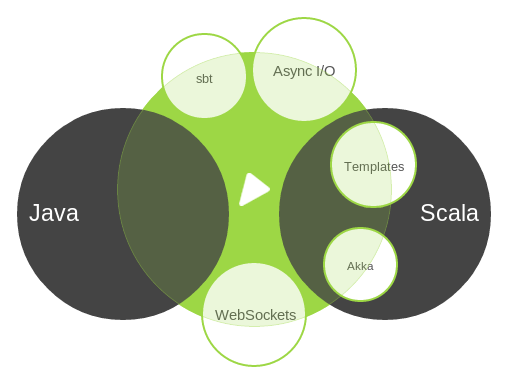
\includegraphics[scale=0.5]{./img/play.png}
\caption{\small{The main attributes and features of the Play! Framework}}
\label{play}
\end{figure}
 
 
The Play! Framework offers excellent documentation\cite{playDoc} that can help us get familiar with the Play! environment. First of all, it is an open source application that has an amazing error handling because of the fact that everything is compiled and built on the fly. This makes it easier for developers to detect bugs and can dramatically improve the developer's productivity to make changes. By reloading the browser, you can immediately see the changes you just made, which makes it perfect for fast prototyping within our project. Moreover, Play! supports both the Scala and Java languages, it comes with a Scala template that allows you to write dynamic code within an HTML body, and it also comes with pre-configured testing support. This last one is particularly important because that means we do not need to worry about adding Junit dependencies to the build file. \\\\
Play! also offers the use of the EBean server interface which is very handy for fetching and saving beans to a particular DataSource. It can make reactive applications simpler because Play! is built on \href{http://netty.io/}{Netty}, which means it supports non-blocking I/O.\footnote{ non-blocking I/O is a form of input/output processing that permits other processing to continue before the transmission has finished.} This will enable our web application to make remote calls inexpensively which is crucial for high performance web applications.

\newpage








% \begin{enumerate}
% 	\item User(Client) interaction with web(Asynchronous vs sync)
% 	\item Distributed application structure(client/server)
% 	\item Scalability is the ability of a system, network, or process to handle a growing amount of work in a capable manner or its ability to be enlarged to accommodate that growth.
% 	\item Build systems
% 	\item Databases(need more research)
% 	\item Continuous Integration
% \end{enumerate}
% \subsubsection{Synchronous Vs Asynchronous}
% \subsubsection{Server-Side Rendering Vs Client/Server}
% \subsubsection{Vertical Scalability Vs. Horizontal Scalability}
% \subsubsection{sbt Vs. Maven}
% \subsubsection{mongodb vs nosql vs mysql vs postgres}
% \subsubsection{Template}
% \subsubsection{Testing}
% \subsubsection{Jenkins}
% \subsubsection{frameworks}



   \section{Conclusion}
  Throughout this report we have first analysed our problem domain to gain more insight into the domain. Secondly we listed the functional requirements, technical requirements and usability requirements. Based on these requirements and problem domain we formulated a research question that would define our research objectives. Finally we have reserached on choosing design patterns and convention for ourselves to deliver an optimal solution for the problem domain.\\\\
MVC model is chosen as design pattern so that components of the system grouped in such a way that has high cohesion and low coupling this will help alot for extension of features. By chosing Play!Framework we are able to use our knowledge in Java and Scala, This enable us to practice Object Oriented Programming as well as Functional programming in this project. We believe by using the finding that we have gained during research phase we can deliver fast,reliable and robust software that acts as an virtual assistant for students.




%%%%%%%%%%%%%%%%ALL Sections ENDS here



%%%%%%%%%%%%%%%%%%%%%%%%%%%%%%%%%%%%%Refrences%%%%%%%%%%%%%%%%%%%%%%%%%%%%%%%%%%%%%%%%%%	
\bibliographystyle{plain}
\bibliography{refrences}


	\end{document}